
\section{Conservative and Non-Conservative Forces\footnote{
1990-93 Dept. of Physics and Astronomy, Dickinson College. Supported by FIPSE
(U.S. Dept. of Ed.) and NSF. Portions of this material may have been modified
locally and may not have been classroom tested at Dickinson College.
}}

\makelabheader %(Space for student name, etc., defined in master.tex or labmanual_formatting_commands.tex)

\medskip
\textbf{Objectives} 

\begin{itemize}[nosep]
\item To investigate the conditions under which mechanical energy is conserved. 
\item To relate conservative and non-conservative forces to the net work done by a
force when an object moves in a closed loop.
\end{itemize}

\medskip
\textbf{Apparatus} 
\begin{itemize}[nosep]
\item Wooden block with hook 
\item Board to use as an incline S
\item 5.0 newton spring scale 
\item Meter stick 
\item Variety of masses 
\item CS2000 compact scale
\item Stop watch
\end{itemize}

\textbf{Introduction }

You already know that mechanical energy is conserved
for a freely falling object. Let's investigate whether mechanical energy is
conserved when an object slides down an inclined plane in the presence of a
friction force.




\textbf{Activity 1: Is Mechanical Energy Conserved for a Sliding Block? }

\begin{wrapfigure}[4]{r}{0.4\textwidth}

\hspace{\fill}
\includegraphics[scale=0.7]{conservative/block_and_ramp.eps}
\end{wrapfigure}

(a) Raise the incline until the block slides at a constant velocity once it
is pushed gently to overcome the static friction force. What is the potential
energy of the block at point A relative to the bottom of the ramp? Show your
data and calculation.
\answerspace{35mm}


(b) What is the potential energy change $\Delta U$ of the block when it reaches point B? Explain.
\answerspace{20mm}

(c) Did the velocity of the block appear reasonably constant as it slid down the ramp?
\answerspace{15mm}

\pagebreak
(d) Assuming the initial kinetic energy (just after your starter shove) is the
same as the final kinetic energy, what is the kinetic energy change, $\Delta K$, of the block when it reaches point B? 
\answerspace{10mm}

(e) Is mechanical energy conserved as a result of the sliding? Cite the evidence for your answer.
\answerspace{20mm}

As you examine the activities you just completed you should conclude that the
conservation of mechanical energy will probably only hold in situations where
there are no friction forces present. 

\textbf{Conservative and Non-Conservative Forces} 

Physicists have discovered that certain conservative forces such as gravitational forces and spring forces do no total work on an object when it moves in a closed loop. Other forces involving friction are not conservative and hence the total work these forces do on an object moving in a closed loop is not zero. In this next activity you will try to determine the validity of this assertion.

%\vspace{0.3cm}
{\par\centering 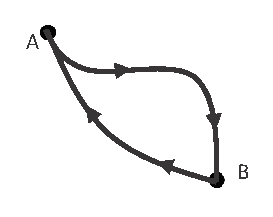
\includegraphics{conservative/two_paths.eps} \par}
%\vspace{0.3cm}

It is not hard to see that a gravitational force does no net work when an object
moves at a constant speed through a complete round trip. In the above figure,
it takes negative external work to lower a mass from point $a$ to point $b$, as
the force of gravity takes care of the work. On the other hand, raising the
mass from point $b$ to point $a$ requires positive external work to be done against the force of gravity, and thus the net work done by the gravitational force
for the complete trip is zero. When a frictional force is present it always
does net work on an object as it undergoes a round trip. For example, when a
block slides from point $a$ to point $b$ on a horizontal surface, it takes work
to overcome the frictional force that opposes the motion. When the block slides
back from point $b$ to point $a$, the frictional force still opposes the motion
of the block so that net work is done. Let's make this idea more concrete by
sliding a block around a horizontal loop on your lab table in the presence of
a frictional force and computing the work it does. Then you can raise and lower
the block around a similar vertical loop and calculate the work the gravitational force does.

\bigskip
\textbf{Activity 2: Are Frictional Forces Conservative According to the Loop
Rule?} 

(a) Put masses on the wooden block and use the spring scale to pull the block
around a rectangular path on your table top at constant velocity. Draw arrows
along the path for the direction of motion and the direction of the friction force exerted on the block. At constant velocity, the friction force will have the same magnitude as the force you measure on the spring scale, but in the opposite direction. List the measured forces and distances for each of the four segments of the path, and calculate the work done by friction around the entire path $a$ to $b$ to $a$ as shown. Remember how we calculated the work done by friction in Activity 2 of  Experiment \ref{work_power}.

\vspace{0.3cm}
{\par\raggedright 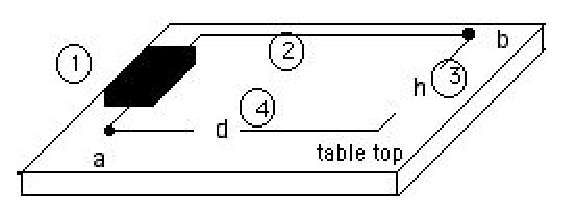
\includegraphics{conservative/conservative_fig3.eps} \par}
\vspace{0.3cm}

\answerspace{20mm}

\hspace{1.5cm}Work (done by friction) around closed loop = \rule{1.5in}{0.1pt}

\answerspace{10mm}

(b) Is the frictional force conservative or non-conservative (i.e., 
is the total work done by the friction force zero or non-zero) according to the loop rule? Explain.
\answerspace{20mm}


Let's return once again to our old friend the gravitational force and apply
an external force to move the same block (without the masses) in a vertical
loop above the table. Be very, very careful to pay attention to the direction
of the gravitational force relative to the direction of the motion. Remember
that work is the dot product of this force and the displacement in each case
so that the work done by the gravitational force when the block moves up and
when it moves down are not the same. What happens to the work when the gravitational force is perpendicular to the direction of motion, as is the case in moving from left to right and then later from right to left?

\vspace{0.3cm}
{\par\centering 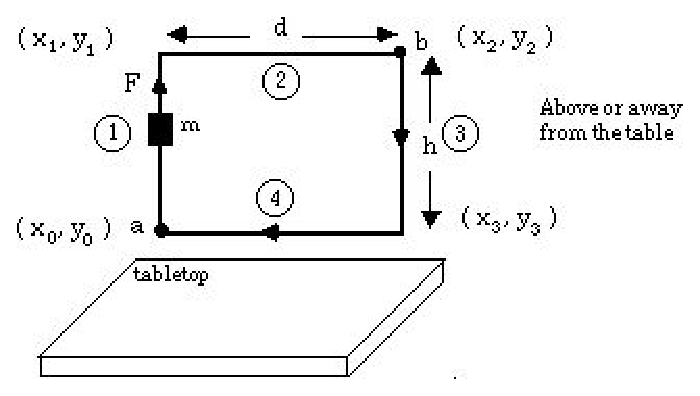
\includegraphics{conservative/conservative_fig4.eps} \par}
\vspace{0.3cm}

%\pagebreak
\textbf{Activity 3: Are Gravitational Forces Conservative? }

(a) Use the spring scale and raise and lower the wooden block around a rectangular
path above your tabletop at a constant speed without allowing it to slide at
all. Draw arrows along the path for the direction of motion and the direction
of the gravitational force exerted on the block. Use your measured distances,
the measurement of the mass of the block and the dot product notation to calculate the work done by the gravitational force on the block over each of the four segments of the path, and over the entire path $a$ to $b$ to $a$ as shown. Be careful not to let the block slide on the table or rub against it. Don't forget to specify the units! Hints: (1) In path 1 
\( \Delta  x
= x_{1}  - x_{0} \), \( \Delta  y = y_{1}  - y_{0} \),
etc. (2) Keep track of the signs. For which paths is the work negative? positive?
\answerspace{40mm}

\hspace{1.5cm}Work (done by gravitational force) around closed loop = \rule{1.5in}{0.1pt}

\answerspace{5mm}

(b) Is the gravitational force conservative or non-conservative according to
the loop rule? Explain.
\answerspace{20mm}

\textbf{The ``Missing'' Energy} 

We have seen in the case of the sliding block (Activity 1) that the Law of Conservation of Mechanical Energy does not seem to hold for forces involving friction. The question is, where does the ``missing'' energy \( \Delta  \)$E$ go when
frictional forces are present? The energy in the system might not all be potential energy or kinetic energy. If we are clever and keep adding new kinds of energy to our collection, we might be able to salvage a Law of Conservation of Energy. If we can, this law has the potential to be much more general and powerful than the Law of Conservation of Mechanical Energy.

\pagebreak[2]
\textbf{Activity 4: What Happens to the Missing Energy?} 

(a) Rub the sliding block back and forth vigorously against your hand? What
sensation do you feel?
\vspace{10mm}

(b) How might this sensation account for the missing energy?
\vspace{20mm}

Physicists call the energy which is lost by a system as a result of work done
against frictional forces thermal energy. This thermal energy may lead to an
increase in the system's internal energy. Using the symbol \(  E_{\rm th} \) to
represent the internal energy of a system that experiences frictional
forces allows us to express the Law of Conservation of Total Energy 
mathematically with the expression
\[E_{\rm sys}=U+K+ E_{\rm th}=\mbox{constant}\]


An alternative way to express energy conservation is to note that when energy
exchanges take place, the total system energy does not change, so that
\[
\Delta E_{\rm sys}=\Delta E_{\rm mech}+\Delta E_{\rm th} = 0\]


We are not prepared in this part of the course to consider the nature of internal energy or its actual measurement, so the Law of Conservation of Energy will
for now remain an untested hypothesis. However, we will re-consider the concept
of internal energy next semester when we deal with heat and temperature.

